% Wczytanie szablonu
\documentclass[nostrict]{Szablon}

% Definicja dokumentu
\usepackage{xcolor}
\usepackage[unicode=true]{hyperref}
\usepackage{array}
\usepackage{float}
\usepackage{changepage}
\usepackage{enumitem}
\newcommand\PDFtitle{Narzędzie do interaktywnego planowania trasy lotu bezzałogowego statku powietrznego}
\newcommand\PDFauthors{Tomasz Krępa, Filip Korthals, Wiktoria Kubacka}
\hypersetup{
  pdftitle={\PDFtitle},
  pdfauthor={\PDFauthors},
}

% Zmiana czcionki dla symulacji maszynopisu (verbatim)
\makeatletter
\renewcommand{\verbatim@font}{\ttfamily\small}
\makeatother

% Część właściwa pracy
\begin{document}
\chapter*{Streszczenie}
% \addcontentsline{toc}{chapter}{Streszczenie}  
\chapter*{Abstract}
% \addcontentsline{toc}{chapter}{Abstract}  
\chapter*{Spis treści}

\tableofcontents

\textcolor{red}{Do oceny rozdział 4.}
\chapter*{Wykaz ważniejszych oznaczeń i skrótów}
\addcontentsline{toc}{chapter}{Wykaz ważniejszych oznaczeń i skrótów}
\chapter{Wstęp i cel pracy (Tomasz Krępa)}
\label{chap:introduction}
W ostatnich latach przemysł samolotów bezzałogowych stał się dostępny dla o wiele szerszej grupy użytkowników. Drony znajdują swoje zastosowanie już nie tylko w przemyśle zbrojeniowym, ale także przemyśle rolniczym, leśnictwie i celach rozrywkowych. Jednym z możliwych sposobów wykorzystania statków bezzałogowych w agrokulturze jest automatyzacja pozyskiwania informacji na temat stanu gleby. W tym celu stosowane są samoloty autonomiczne typu fixed-wing, które mają większe możliwości w zakresie odległości i czasu lotu niż standardowe drony, jednak nie są w stanie wykonywać takich samych manewrów co standardowe drony wykorzystywane komercyjnie, np. w fotografii. Obecnie ciężko jest znaleźć rozwiązania pozwalające na przystępne wyznaczanie obszaru i trajektorii przelotu samolotów tego typu. Większość implementacji nie skupia się w wystarczającym stopniu na wyznaczaniu obszaru i pozostawia tę część rozwiązania użytkownikowi. 

Motywacją do realizacji tego projektu jest możliwość rozwoju technologii wspierającej agrokulturę i leśnictwo. Automatyzacja w tak ważnych ekologicznie obszarach jest w dzisiejszych czasach bardzo istotna. Możliwość zoptymalizowanego badania stanu gleby rolnej lub wilgotności ściółki leśnej pozwoli na usprawnienie procesów hodowli roślin czy informacji przeciwpożarowej. Patrząc na pozytywne skutki wykorzystania samolotów bezzałogowych w tych obszarach, można niezaprzeczalnie stwierdzić, że jest to technologia zasługująca na rozwój.

Celem niniejszego projektu dyplomowego jest stworzenie aplikacji internetowej pozwalającej na planowanie trasy przelotu drona na podstawie satelitarnych zdjęć terenu. Zaimplementowane zostaną algorytmy wykrywania krawędzi oraz wytyczania krzywych zakreślających zadany obszar. Aplikacja zostanie wykonana przy wykorzystaniu środowisk Next.js i Python.

W drugim oraz trzecim rozdziale omówione zostały zagadnienia zgłębiające dalej dziedzinę, której poświęcamy naszą pracę. Autorem rozdziału czwartego jest XX, w którym przedstawia on aktualny stan wiedzy i technologii dotyczącej naszego rozwiązania. Autorami rozdziału piątego są YY i XX. Sekcja ta poświęcona jest analizie naszego systemu. Podrozdziały napisane przez YY są poświęcone dokładnej specyfikacji postawionych przed nami wymagań projektowych, a pozostałe podsekcje, autorstwa XX, przedstawiają nasz zespół, harmonogram prac nad implementacją oraz analizują ryzyka związane z realizacją przedsięwzięcia informatycznego. W szóstym rozdziale, XX opisał projekt naszego systemu, a w szczególności przeznaczenie użytkowania produktu, koncepcje naszych rozwiązań a także projekty poszczególnych komponentów wykorzystanych w finalnym narzędziu. Autorem siódmego rozdziału jest XX i ta część pracy poświęcona jest implementacji a także testom i weryfikacji możliwości naszej aplikacji w środowisku docelowym. Rozdział ósmy, którego autorem jest XX, poświęcony został naszym wynikom i wnioskom wyciągniętych w trakcie realizacji projektu. W tej części zawarte zostały także możliwości i pomysły dalszego rozwoju narzędzia. 
\chapter{Wprowadzenie do dziedziny}
\label{chap:field}
\chapter{Stosowana terminologia}
\label{chap:terminology}

\begin{description}
   \item Google Maps --- narzędzie oferowane przez firmę Google umożliwiające przeglądanie map oraz zaznaczanie punktów na nich 
   \item API (ang. \textit{application programming interface}) --- interfejs służący do komunikacji pomiędzy podprogramami systemu lub z systemami zewnętrznymi
   \item UAV (ang. \textit{unmanned aerial vehicle}), dron --- bezzałogowy statek powietrzny, samolot niewymagający do lotu załogi na jego pokładzie
   \item CPP (ang. \textit{coverage path planning}), planowanie ścieżki pokrycia --- problem informatyczno-robotyczny polegający na wytyczeniu ścieżki przez obszar oferującej jak największe i najbardziej optymalne pokrycie tego obszaru
\end{description}
\chapter{Istniejące rozwiązania (Filip Korthals)}
\label{chap:example solutions}

W niniejszym rozdziale przedstawiono przykładowe rozwiązania zbliżone do problemu opisywanego w tej pracy.

\section{Aplikacja do planowania trasy drona - PIX4Dcapture}

PIX4Dcapture to aplikacja mobilna szwajcarskiej firmy Pix4D, udostępniająca mapy offline oraz planowanie trasy, które odbywa się za pomocą nanoszonych obszarów misji na mapę \cite{pix4dcapture}. Istnieje w niej także możliwość planowania siatki trasy oraz torów eliptycznych lub manualnego sterowania, aby przyjrzeć się danemu obiektowi. Na ich podstawie aplikacja wyznacza trasę dla drona przebiegającą po wybranym obszarze mającym z góry zdefiniowany tor ruchu. Głównym celem jest sfotografowanie całego terenu przez drona, aby następnie za pomocą innych narzędzi wykorzystać wykonane zdjęcia i dokonać mapowania terenu – w 2D lub 3D. Stosowane również jako przydatne narzędzie przy modelowaniu obiektów. Aplikacja jest dostępna na systemy Android i iOS, ale również na wybrane kontrolery do dronów. Co istotne, połączenie sieciowe nie jest wymagane podczas korzystania z aplikacji, więc nie ma problemu przy wykonywaniu przelotów w obszarach o słabym zasięgu sieci.

System oferowany przez Pix4D daje możliwość wybrania modelu drona, aby po zaplanowaniu trasy móc wgrać ją bezpośrednio do pamięci statku powietrznego. Aplikacja nie wspiera wszystkich dronów, kamer i kontrolerów, a ich lista jest określona w dokumentacji dostarczonej przez producenta \cite{pix4dcapture_supported}. Chcąc skonfigurować planowanie trasy, użytkownik jest proszony o wybór rodzaju misji. Każdy rodzaj ma inne zastosowanie i wyznacza, w jaki sposób dron będzie się przemieszczał po wybranym terenie. Najbardziej typowym rodzajem misji i sprawdzającym się w większości przypadków jest opcja \textit{Grid}, która tworzy trasę na kształt siatki w prostokątnym obszarze. Ma to zastosowanie przy mapowaniu dwuwymiarowym i tylko w przypadku pól prostokątnych. Do mapowania pól o nieregularnych kształtach została dodana opcja \textit{Polygon}, która umożliwia dostosowanie krawędzi nanoszonego obszaru do faktycznych granic pola. Następnie na wyznaczony obszar, podobnie jak w poprzednim przypadku, zostaje naniesiona siatka, po której ma poruszać się dron. Kolejnym rodzajem misji jest \textit{Double Grid}, który działa podobnie do zwykłego \textit{Grid}, przy czym na obszar nanoszone jest więcej siatek niż tylko jedna. Ma to na celu wykonanie zdjęć terenu z różnych stron, aby zebrać detale widoczne też w pionie, a nie tylko w poziomie. Takie podejście ma zastosowanie przy trójwymiarowym mapowaniu terenu. Z tego powodu, producent zaleca stosowanie tego trybu do latania w małej odległości od mapowanych obiektów \cite{pix4d_missions}. Następnym rodzajem misji jest misja \textit{Circular}, stworzona do dokładnego fotografowania obiektów ze wszystkich stron. Obszar należy umieścić tak, aby mapowany obiekt znajdował się w jego centrum. Dron podążający wyznaczoną trasą powinien obracać się równomiernie z zataczaniem okręgu wokół celu. W przypadku fotografowania obiektów wysokich – przykładowo wieżowców – producent zaleca wykonanie wielu takich misji na różnych wysokościach. Ostatni rodzaj misji nazywa się \textit{Free Flight} i został on stworzony do najbardziej skomplikowanych celów, do których nie pasuje żaden z uprzednio wymienionych trybów. W tym przypadku nie jest wyznaczana trasa, a pilot musi samodzielnie sterować dronem. Natomiast dzięki aplikacji PIX4Dcapture, zdjęcia są wykonywane automatycznie po przebyciu przez drona określonego dystansu – w pionie i poziomie.

\begin{figure}[H]
    \centering
    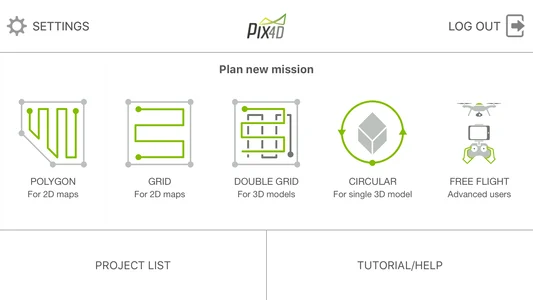
\includegraphics[width=\textwidth]{images/PIX4D_Wybor_misji.png}
    \caption{Wybór rodzaju misji}
\end{figure}

Parametry misji można dowolnie dostosowywać do własnych potrzeb. Można zarówno manipulować rozmiarem, jak i rotacją wybranego obszaru. Użytkownik ma możliwość dostosowania wysokości lotu oraz prędkości, z jaką dron ma się poruszać. Wybraną misję z konkretnymi ustawieniami można zapisać, aby wykorzystywać ją wielokrotnie w przyszłości.

\begin{figure}[H]
    \centering
    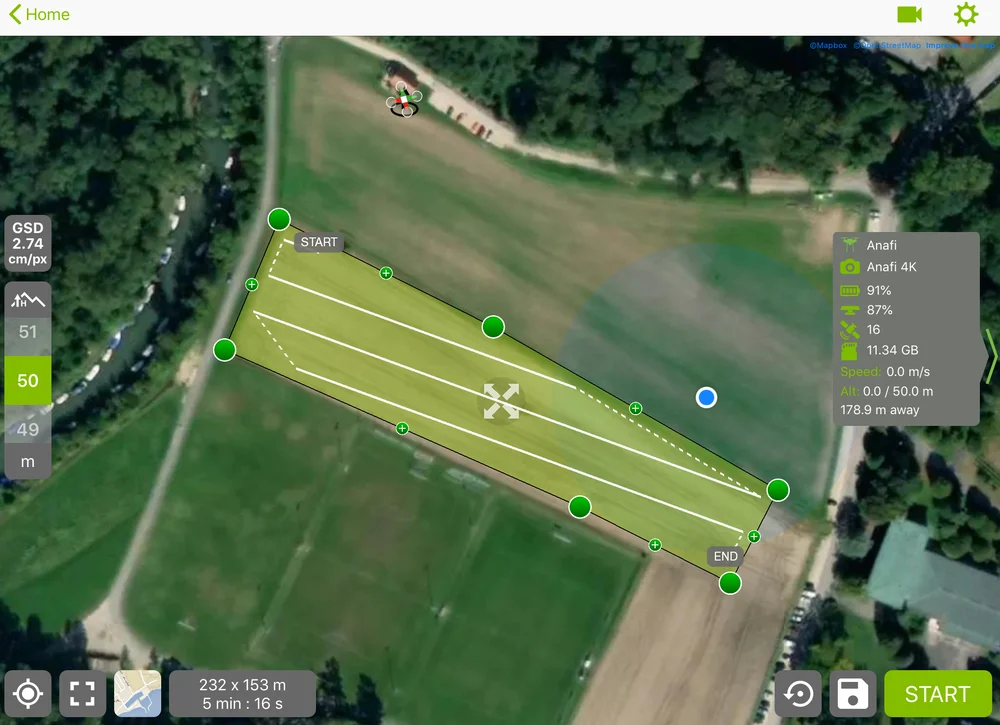
\includegraphics[width=\textwidth]{images/PIX4D_Przebieg_misji.png}
    \caption{Wybrana misja}
\end{figure}

Kolejnym krokiem jest już połączenie aplikacji z dronem i wgranie do pamięci urządzenia zaplanowanej trasy. Z poziomu aplikacji można wykonać start misji, po którym dron automatycznie wystartuje i wykona wgraną trasę. Zdjęcia również są wykonywane automatycznie, więc użytkownik musi jedynie kontrolować, czy wszystko przebiega zgodnie z planem. Po wykonanej misji dron sam wraca na miejsce startu. Wykonane fotografie można następnie przenieść do innych narzędzi służących do mapowania terenu, które producent również oferuje. Przy korzystaniu w tym celu z aplikacji od Pix4D, powstał format pliku .p4d, który bardzo ułatwia przenoszenie danych między aplikacjami i późniejszą pracę nad projektem.

Producent nie dostarcza zbyt wielu informacji na temat swojego produktu poza dokumentacją zawierającą dane o funkcjonalnościach systemu. Jest to przydatne narzędzie do planowania trasy, ale w konkretnym celu – w celu mapowania i modelowania. W przypadku problemu przedstawianego w niniejszej pracy, kiedy istotny jest aspekt skupienia się na konkretnym obszarze pola oraz najbardziej optymalnego wykorzystania baterii do pokrycia całego pola, aplikacja PIX4DCapture nie przynosiłaby zadowalających rezultatów.

\section{Aplikacja do kontroli lotu drona – Dronelink}

Dronelink to aplikacja umożliwiająca kontrolowanie lotu drona manualnie lub automatycznie i wyznaczanie trasy na mapie po z góry zdefiniowanym przez użytkownika obszarze. Pozwala ona też na pobieranie danych podczas lotu. Aplikacja jest dostępna zarówno w internecie, jak i na urządzenia mobilne oraz niektóre kontrolery do dronów. Jej celem jest pomoc przy fotografowaniu terenu lub obiektów w różnych celach – od hobbystycznych do profesjonalnych. Stąd grupą docelową produktu jest każdy użytkownik drona, który ma potrzebę realizowania precyzyjnych i powtarzalnych lotów.

Główną funkcjonalnością aplikacji jest planowanie trasy na podstawie nanoszenia szablonu \cite{dronelink}. Użytkownik jest proszony o wskazanie miejsca na mapie i naniesienie w dane miejsce szablonu dostarczonego przez producenta. Naniesiony wzór można dowolnie modyfikować pod swoje potrzeby. Możliwa jest ręczna konfiguracja rozmiaru pokrywanego obszaru, jego kształtu, kierunku planowanej trasy i miejsca startu czy lądowania drona. Aplikacja umożliwia również dostosowanie przebiegu trasy do ukształtowania terenu, co jest nietypowym rozwiązaniem w porównaniu do konkurencji. Przechodząc do kolejnych parametrów – użytkownikowi udostępniane są opcje modyfikacji już samego lotu – wysokość i prędkość przelotu czy kąt nachylenia kamery. To tylko część z oferowanych ustawień, ponieważ system ma ich wiele z racji na bardzo szeroki zakres możliwości jego wykorzystania. Po zapisaniu trasy, jest ona dostępna w bibliotece przypisanej do konta, więc można uzyskać do niej dostęp na każdym urządzeniu po zalogowaniu. Taką trasę można wgrać do pamięci statku powietrznego, który automatycznie wykona trasę. Dron jednak nie pozostaje jednak bez kontroli i pilot może w każdej chwili zatrzymać misję i przejąć kontrolę, w tym wywołać komendę powrotu drona na miejsce startu. Ma to zastosowanie choćby przy długich trasach. Drony często mają taką baterię, która nie pozwala na długi czas lotu. W takiej sytuacji pilot może przerwać misję, aby wymienić baterię i następnie wznowić lot. Aplikacja zapamiętuje miejsce, w którym została zatrzymana misja i po jej wznowieniu dron automatycznie wraca na miejsce przerwania, aby od tego miejsca zacząć dalsze fotografowanie według planu.

Wspomnianych szablonów producent zapewnia kilka podstawowych rodzajów, aby użytkownik mógł znaleźć wzór najbardziej dopasowany do swoich potrzeb. Pierwszym szablonem jest \textit{Map}, który jest przeznaczony do mapowania terenu. Działa na bardzo podobnej zasadzie jak w przypadku aplikacji PIX4Dcapture – na wyznaczony obszar nanoszona jest siatka, która umożliwi dronowi ujęcie kamerą całego oczekiwanego terenu. Kolejnym szablonem jest \textit{Waypoints}, który już nie ma na celu mapowania terenu, ale wyznaczenie ścieżki, którą ma przebyć dron, na podstawie naniesionych punktów orientacyjnych. Użytkownik może dowolnie dodawać i usuwać punkty, kształtować trasę między nimi lub konfigurować zachowanie drona na poszczególnych etapach lotu. Jest to wzorzec skierowany choćby do filmowców, aby uzyskać przelot, który będzie dokładnie spełniał wszystkie wymaganie i będzie przy tym mocno powtarzalny. Następnym szablonem, również istniejącym u konkurencji od firmy Pix4D, jest \textit{Circle}, który oferuje trasę krążenia wokół wybranego celu. To również może posłużyć do mapowania, ale już nie w poziomie, a w pionie – zwłaszcza konkretnych obiektów. Ostatnim oferowanym szablonem jest \textit{Pano}, które pozwala na utworzenie zdjęcia panoramicznego. Na podstawie zaplanowanej trasy dron wykonuje serię zdjęć, które następnie są łączone w jedno, spójne zdjęcie panoramiczne. Zdjęcie może być zarówno poziome, jak i pionowe. W aplikacji są dostępne jeszcze inne, zaawansowane szablony misji. Te trasy są już bardziej złożone i przeznaczone do bardziej specyficznych celów – raczej rzadko używane. Są to pewne konfiguracje tras podstawowych, ale na pewno daje to wygodę użytkownikowi, aby skorzystać ze złożonych szablonów zamiast ręcznie konfigurować szablon podstawowy.

Ciekawymi funkcjami przy planowaniu trasy są przegląd 3D oraz symulacja trasy. Przegląd 3D umożliwia obejrzenie zaplanowanej trasy ze wszystkich stron, a nie tylko w rzucie z góry przy standardowym patrzeniu na mapę. Pomaga to zobrazować zmiany w wysokościach lotu w poszczególnych momentach misji. Symulacja trasy natomiast pozwala sprawdzić przebieg całej trasy bardzo szczegółowo. Generowany jest wirtualny lot, w tym obraz na podstawie zdjęć satelitarnych z przewidywanym rezultatem, który może uzyskać dron. Są przy tym wyświetlane wszystkie parametry, takie jak: prędkość chwilowa, wysokość oraz przebyta droga. Dla jeszcze większej kontroli dodana jest oś czasu, która obrazuje co dokładnie się wydarzy w którym momencie lotu.

\begin{figure}[H]
    \centering
    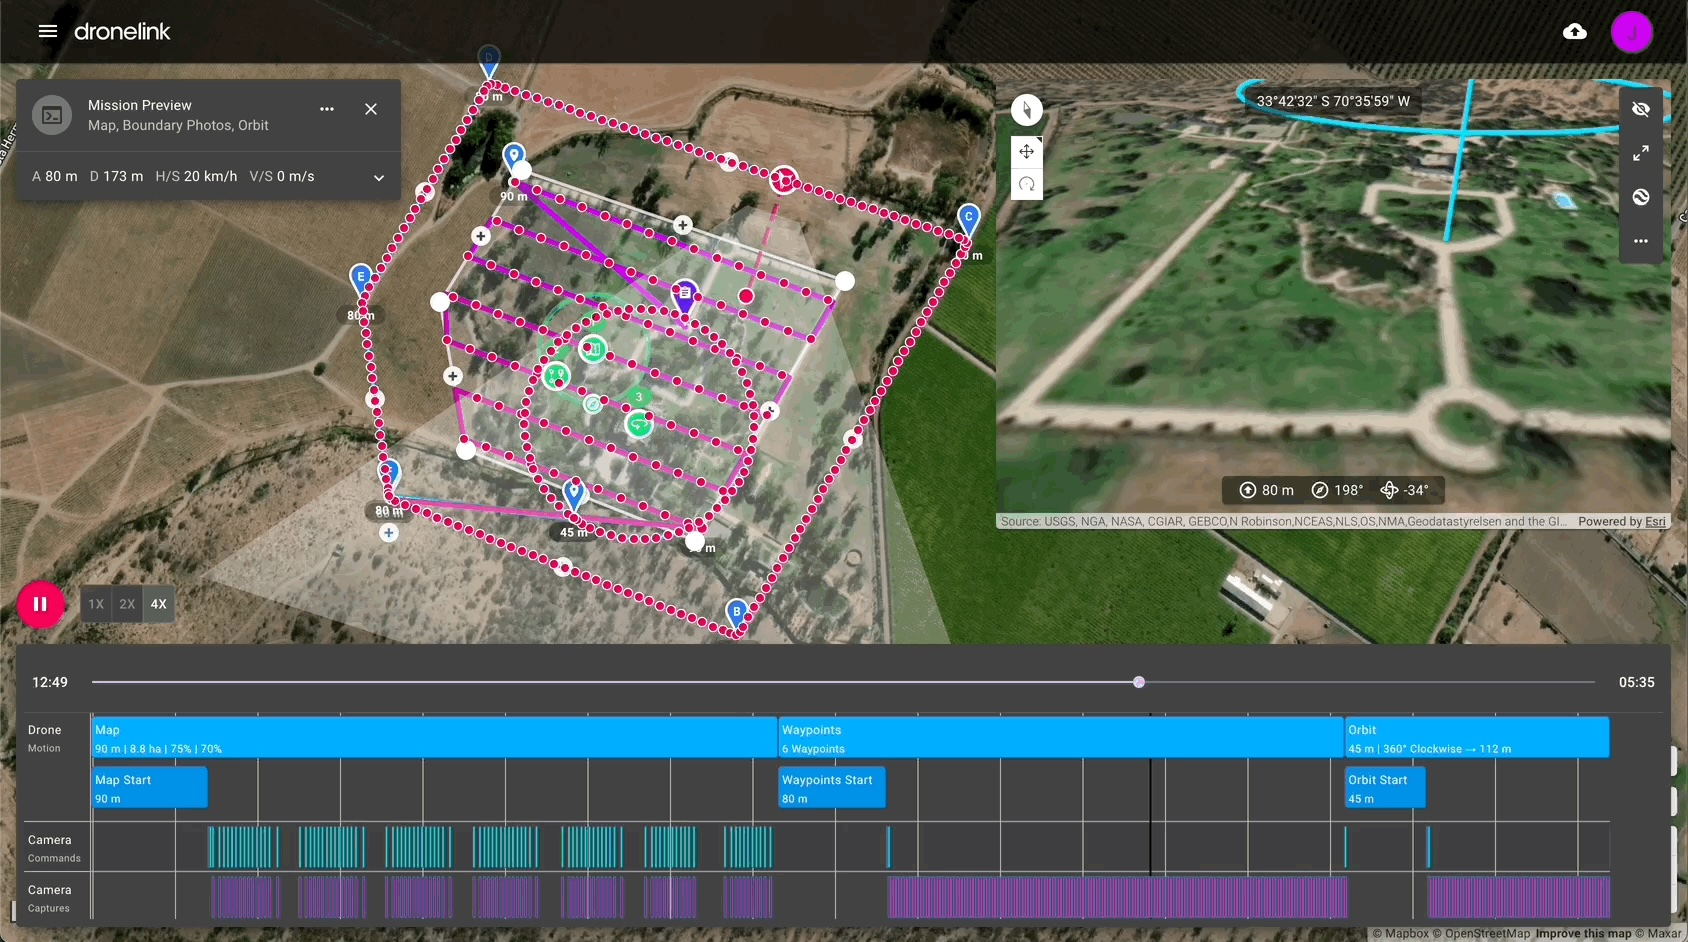
\includegraphics[width=\textwidth]{images/Dronelink_symulacja.jpg}
    \caption{Symulacja misji}
\end{figure}

Dronelink oferuje również inne tryby pracy, nie tylko planowanie tras z szablonów. Jednym z nich jest tryb misji \textit{On-the-fly}. Takie misje dają użytkownikowi wskazówki do wykonania konkretnych manewrów dronem, aby wytyczyć parametry do generowania trasy. Jednym typem takiej misji – bardziej opisanym przez producenta – jest \textit{On-the-fly Waypoints}. Polega on na wyznaczaniu punktów orientacyjnych za pomocą drona. Użytkownik łączy drona z aplikacją i ręcznie wykonuje lot. Następnie w aplikacji zaznacza miejsca, w których dron się akurat znajduje. W ten sposób użytkownik sam wybiera punkty, na których mu zależy. Dzięki temu, punkty mogą być wskazane na podstawie faktycznego widoku z kamery, a nie tylko położenia na mapie, które może być niewystarczającym wyznacznikiem położenia oczekiwanego kadru. W dalszej fazie z wyznaczonych punktów orientacyjnych zostaje wytyczona trasa, którą można modyfikować tak samo, jak w przypadku trasy z szablonu.

\begin{figure}[H]
    \centering
    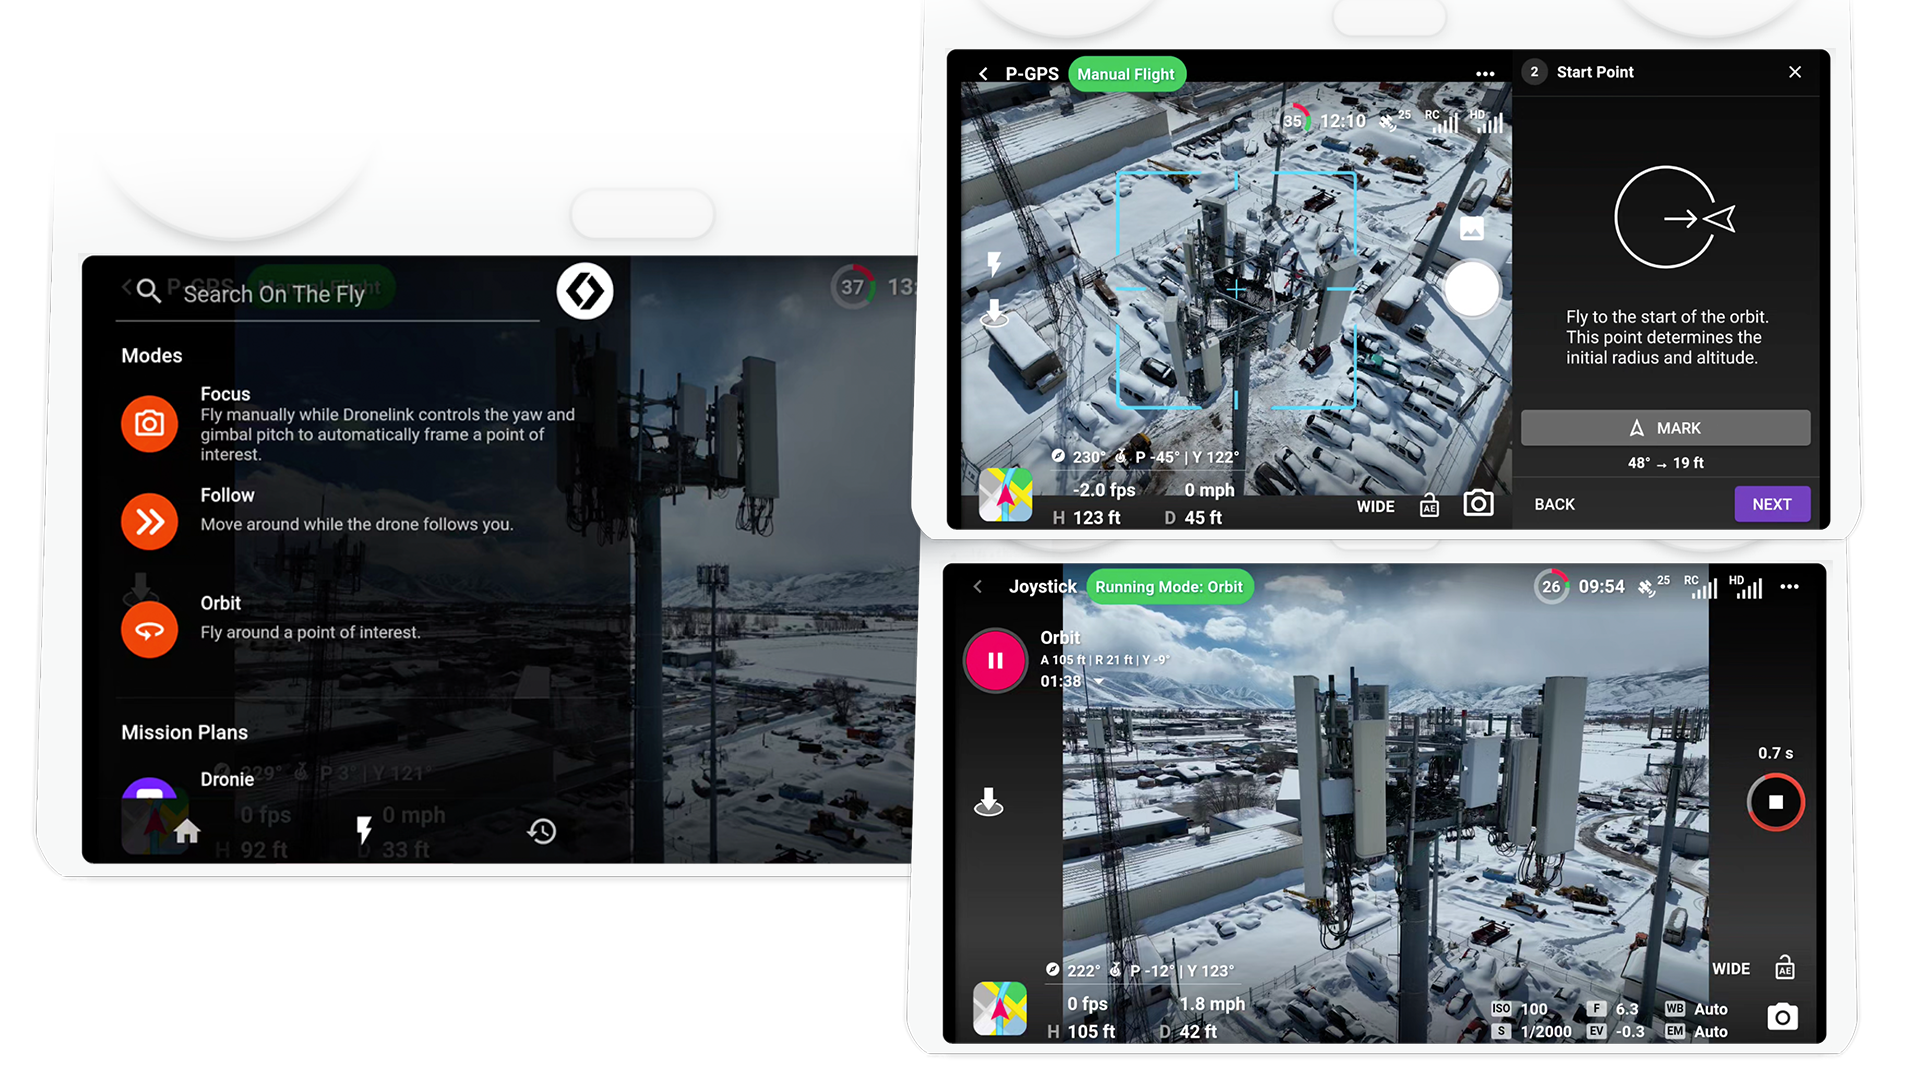
\includegraphics[width=\textwidth]{images/Dronelink_misje_hybrydowe.png}
    \caption{Przegląd misji hybrydowych}
\end{figure}

Trzeci i ostatni tryb pracy determinuje tryb lotu drona. Są to misje hybrydowe, czyli część działań jest wykonywana automatycznie, a część jest pozostawiona kontroli użytkownika. W ten sposób użytkownik ma kontrolę nad działaniami drona, ale ta praca jest uproszczona, więc można się skupić na tym, na czym najbardziej użytkownikowi zależy. W tym trybie oferowane są trzy rodzaje lotów: \textit{Focus}, \textit{Follow} i \textit{Orbit}. Pierwszy z wymienionych daje użytkownikowi swobodę w sterowaniu dronem, ale pomaga przy ujęciach wybranego celu. Wymagane do tego jest ustawienie celu, którego użytkownik chce wykonać zdjęcia. Następnie, podczas lotu, dron automatycznie będzie się obracał i kierował kamerę na wybrany wcześniej cel. Użytkownik może dynamicznie dobierać miejsce, z którego ma być wykonane ujęcie, bez jednoczesnego zajmowania się ustawianiem kamery. Drugi rodzaj lotu z wymienionych, czyli \textit{Follow}, wprowadza funkcję śledzenia użytkownika. Dron na bieżąco podąża za urządzeniem z aplikacją Dronelink oraz dostosowuje kamerę tak, aby cel znajdował się w centrum. Istnieje przy tym kilka opcji dostosowania parametrów lotu do swoich potrzeb. Są to: ustawienia korzystania z kontrolera do korekcji położenia drona, ustawienie dynamicznego punktu lądowania – aby dron wrócił do użytkownika zamiast do miejsca startu, automatyczne dostosowywanie wysokości lotu do ukształtowania terenu oraz automatyczny start nagrywania. Ostatni rodzaj lotu – \textit{Orbit} – łączy cechy misji \textit{Circle} oraz \textit{Focus}. Użytkownik jest proszony o wyznaczenie punktów określających obiekt, który ma być fotografowany. Następnie, po podaniu wszystkich wymaganych parametrów, generowana jest trasa, według której dron orbituje wokół obiektu. Użytkownik w trakcie lotu ma pełną kontrolę nad dronem i może za pomocą kontrolera na bieżąco modyfikować lot. 

Aplikacja Dronelink oferuje opcję integracji z innymi systemami w celu wygodniejszej pracy nad uzyskanymi danymi. Producent na swojej stronie opisuje współpracę swojego produktu z systemami WebODM, Airdata oraz Pix4D. W przypadku dwóch ostatnich, aplikacja umożliwia bezpośrednie połączenie systemów w celu szybszego i łatwiejszego przesyłania danych.

Opisywany system jest dostępny na przeglądarki internetowe, niektóre kontrolery oraz urządzenia mobilne z systemem Android i iOS tworząc w ten sposób wysoką dostępność produktu dla użytkownika. Zakres obsługiwanych dronów jest już bardziej ograniczony. Pełna lista jest dostępna na stronie producenta \cite{dronelink_supported}. Są to w większości urządzenia producenta DJI. Jest to popularna marka dronów, ale wciąż dla posiadaczy urządzeń od innych producentów stanowi to jakieś ograniczenie. Natomiast od strony wsparcia technicznego, producent udostępnia stronę internetową z licznymi poradnikami. Są wśród nich instrukcje używania poszczególnych funkcjonalności, w tym nagrania wideo z komentarzem. Niestety producent nie dostarcza żadnej dokumentacji technicznej do produktu. Niektóre komponenty są opisane jedynie powierzchownie, a poradniki dotyczą tylko wybranych elementów. Nawet dosyć szczegółowe poradniki nie opisują dokładnie każdego elementu, a jedynie podstawowy sposób użycia danej funkcjonalności. Z tego powodu trudno jest dotrzeć do wszystkich szczegółów na temat aplikacji bez jej zakupu.

Dronelink jest produktem płatnym, dostępnym w planach subskrypcyjnych lub płatnych jednorazowo. Pojedynczy zakup dotyczy planów hobbystycznych – do celów rekreacyjnych, edukacyjnych i non-profit. W ofercie są trzy takie plany. Najtańszy jest plan podstawowy, a pozostałe – odpowiednio droższe – stanowią kolejne rozszerzenia tego planu. Analogicznie sytuacja się prezentuje w przypadku subskrypcji. Plany te są skierowane do celów profesjonalnych, komercyjnych. Zawierają one już bardzo zaawansowane narzędzia, dodatkowe opcje dostosowania oprogramowania do własnych potrzeb oraz zapewnione wsparcie producenta. Plany subskrypcyjne umożliwiają rozliczenie roczne lub miesięczne. Dzięki tak wielu opcjom zakupu dostępu do produktu użytkownik może wybrać plan najbardziej zbliżony do swoich potrzeb bez konieczności przepłacania za nadmiarowe funkcje, z których nie skorzysta.
\include{chapters/5_przegląd_stanu_wiedzy}
\chapter{Analiza systemu}
\label{chap:system analysis}

W tym rozdziale są wymienione i opisane wszystkie wymagania, jakie zostały postawione przed implementacją aplikacji do planowania trasy dla bezzałogowego statku powietrznego. Ponadto są tutaj zamieszczone informacje o zespole oraz harmonogram pracy i analiza ryzyk jakie mogą wystąpić w projekcie.

\section{Specyfikacja wymagań}

Aplikacja internetowa mająca na celu wyznaczanie trasy dla bezzałogowego statku powietrznego zbierającego dane z czujników umieszczonych w ziemi. Trasa przelotu jest wyznaczona na podstawie wybranych przez użytkownika punktów na mapie tak, aby jak najlepiej pokrywała wybrany teren leśny lub pole. Granice obszaru, który ma zostać pokryty obejmują zaznaczone miejsca i zostają wyznaczone na podstawie zdjęć satelitarnych. Wynikiem działania programu ma być wizualizacja wyznaczonej trasy na mapie przechodzącej przez wybrane punkty.

\subsection{Wymagania funkcjonalne}
Jedną z części specyfikacji wymagań są wymogi dotyczące funkcji i działania systemu. Na podstawie założeń wynikających z natury projektu wybrane zostały następujące wymagania funkcjonalne: 
\begin{itemize}
    \item odczyt współrzędnych geograficznych punktów wskazanych przez użytkownika,
    \item odczyt prędkości lotu drona i maksymalnego czasu przelotu (prędkość z zakresu 50-120\,km/h, maksymalny czas przelotu z zakresu 1-2\,h),
    \item wyznaczanie granic obszaru leśnego lub pola rolnego na podstawie zdjęcia satelitarnego,
    \item wyznaczanie obszaru jaki ma zostać pokryty przez przelot drona na podstawie zaznaczonych punktów na mapie oraz wyznaczonych granic ze zdjęcia satelitarnego,
    \item wyznaczanie optymalnej trasy na podstawie wyznaczonego obszaru, punktów, danych podanych przez użytkownika oraz założonych stałych promienia zasięgu drona i czasu wymaganego na przesył danych,
    \item wizualizacja wyznaczonej trasy.
\end{itemize}

\subsection{Wymagania dotyczące warstwy interakcji z użytkownikiem}

Poniżej znajdują się wymagania dotyczące warstwy interakcji z użytkownikiem: 

\begin{itemize}
    \item nauka obsługi interfejsu nie zajmuje więcej niż pięciokrotne przeprowadzanie procesu planowania trasy,
    \item interfejs responsywny dla urządzeń mobilnych,
    \item interfejs zawiera pola do wprowadzenia parametrów lotu oraz nie daje możliwości wprowadzenia niepoprawnych danych,
    \item interfejs korzysta z API Google Maps.
\end{itemize}

\subsection{Wymagania systemowe}
Aplikacja powinna działać na urządzeniach z dostępem do przeglądarki internetowej oraz połączenia sieciowego. 

\subsection{Wymagania niefunkcjonalne}

Poniżej znajdują się wymagania niefunkcjonalne, jakie powinna spełniać ta aplikacja:

\begin{itemize}
    \item konfigurowalność -- system powinien mieć możliwość zmiany parametrów przelotu drona: czasu lotu oraz prędkości przelotowej,
    \item przenośność -- system powinien działać na zarówno na urządzeniach przenośnych, jak i komputerach stacjonarnych,
    \item kompatybilność - system powinien działać na najpopularniejszych przeglądarkach w aktualnie najnowszych, stabilnych wersjach.
\end{itemize}

\section{Kryteria akceptacji}

Kryteria, które są niezbędne, aby projekt został uzany za zakończony:

\begin{itemize}
    \item pobieranie parametrów lotu od użytkownika,
    \item możliwość wyśrodkowania mapy w wyszukanym miejscu,
    \item możliwość nanoszenia wybranych punktów na mapę,
    \item wykrywanie krawędzi pól lub lasów, na których znajdują się wskazane punkty,
    \item wyznaczanie trasy na podstawie wskazanych punktów oraz parametrów,
    \item informacja zwrotna w przypadku braku możliwości pokrycia zaznaczonego przez użytkownika terenu przez przelot drona,
    \item wyznaczona przez program trasa jest możliwa do wykonania przez danego drona oraz znajduje się w wyznaczonym obszarze,
    \item wizualizacja przebiegu poprawnej trasy.
\end{itemize}

\section{Zespół projektowy}

Zespół projektowy składa się z trzech osób:

\begin{itemize}
    \item Wiktoria Kubacka -- studenkta
    \item Tomasz Krępa -- student
    \item Filip Korthals -- student
\end{itemize}

\section{Harmonogram pracy}

\renewcommand{\arraystretch}{1.5}
\begin{tabular}{ | p{8cm} | p{4cm}| } 
  \hline
  \textbf{Miesiąc} & \textbf{Zadanie} \\
  \hline
  przegląd literatury & marzec \\ 
  \hline
  wybór technologii & marzec \\ 
  \hline
  specyfikacja wymagań & marzec \\ 
  \hline
  implementacja interfejsu użytkownika & kwiecień \\
  \hline
  wykrywanie krawędzi na mapach & kwiecień \\
  \hline
  implementacja planowania trasy & maj \\
  \hline
  wizualizacja wyników & maj \\
  \hline
  planowanie zakończenie implementacji & czerwiec \\
  \hline
  udoskonalanie implementacji & październik-listopad \\ 
  \hline
  dokończenie i udoskonalanie dokumentacji & październik-listopad \\
  \hline
  
\end{tabular}

\section{Analiza ryzyka}


\chapter{Projekt systemu (Wiktoria Kubacka)}
\label{chap:system project}

Poniżej znajduje się projektu systemu będącego aplikacją do planowania trasy dla bezzałogowego statku powietrznego. Zostały tutaj umieszczone cele i przeznaczenie systemu, a także koncepcja rozwiązania. Wykonany projekt obejmuje architekturę systemu, diagram przypadków użycia, diagram klas a także projekt interfejsu użytkownika. 

\section{Cel i przeznaczenie systemu}

Celem systemu jest optymalne wyznaczanie trasy przelotu z uwzględnieniem zadanych parametrów tak, by w możliwie optymalny sposób pokryć teren leśny lub rolny wybrany przez użytkownika. Aby to było możliwe, aplikacja musi wyznaczyć dany obszar na mapie wykorzystując wykrywanie krawędzi.

\section{Koncepcja rozwiązania}



\section{Projekt poszczególnych elementów systemu}

W poniższych sekcjach zostały przedstawione diagramy wraz z opisami ilustrujące działanie systemu oraz jego strukturę. Ponadto, zostanie uzasadniony wybór środowiska oraz wykonanej implementacji.

\subsection{Projekt architektury systemu}

Projekt architektury systemu obejmuje dwie główne części składowe widoczne na schemacie. Ponadto, w projekcie zostało uwzględnione wykorzystanie zewnętrznych API do pobierania danych potrzebnych do działania aplikacji. Jedną z części aplikacji jest frontend, obejmujący implementację interfejsu wykorzystywanego do komunikacji z użytkownikiem i prezentowania wyników działania. Wykorzystane zostało tutaj zewnętrzne API Google Maps, które pozwoli na wybór odpowiedniego obszaru i zaznaczanie punktów przez użytkownika, a także prezentację otrzymanych wyników na rzeczywistym obrazie. Drugą częścią jest backend odpowiedzialny za obsługę żądań oraz wykrywanie obszarów na mapach i planowanie trasy. Ta część systemu będzie wykorzystywała Google Earth Engine API do pobierania zdjęć satelitarnych oraz wykonywania na nich operacji.

\begin{figure}[H]
    \centering
    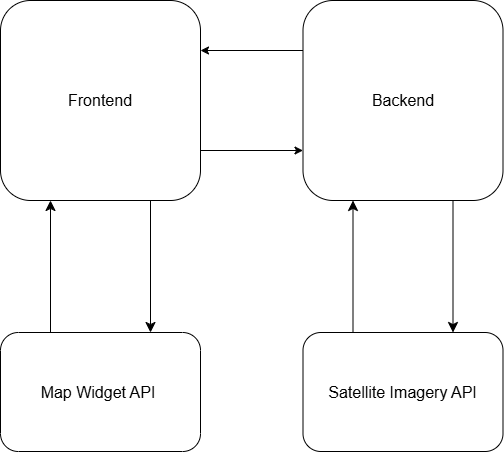
\includegraphics[width=10cm]{images/Architektura_systemu.png}
    \caption{Architektura systemu}
\end{figure}

Na powyższym schemacie widać relacje, jakie zachodzą między poszczególnymi elementami systemu. Frontend będzie wykorzystywał pobrany z API Google Maps komponent mapy, a także będzie wykonywał żądania do backendu w celu zaplanowania trasy dla zadanego terenu. Backend będzie obsługiwał te żądania z wykorzystaniem API Google Earth Engine i zwracał potrzebny wynik do interfejsu w celu zaprezentowania wyników użytkownikowi.

\subsection{Diagram przypadków użycia}

Poniżej został przedstawiony diagram przypadków użycia ilustrujący działanie systemu oraz jego granice, a także opisy każdego z przypadków użycia.

\begin{figure}[H]
    \centering
    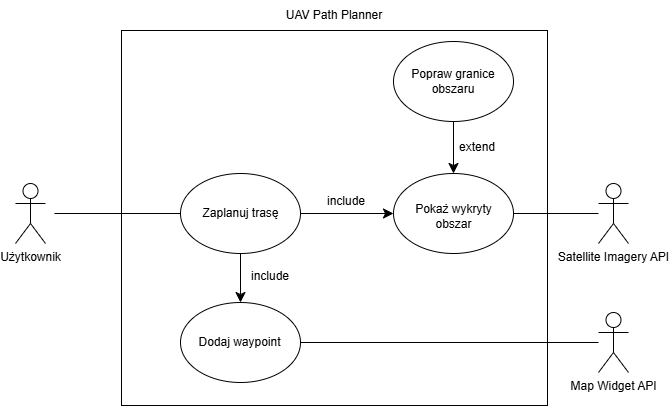
\includegraphics[width=15cm]{images/Diagram_przypadków_użycia.png}
    \caption{Diagram przypadków użycia}
\end{figure}

\hypertarget{plan route}{\textbf{Zaplanuj trasę}} \\*

\textit{Warunki początkowe}

Brak \\*

\textit{Scenariusz interakcji}
\begin{enumerate}
    \item Użytkownik wprowadza prędkość przelotową drona oraz maksymalny czas lotu drona.
    \item Użytkownik wyszukuje na mapie odpowiednie miejsce i wybiera opcję dodania nowego punktu.
    \item Następuje przejście do przypadku użycia \hyperlink{add waypoint}{dodaj waypoint}.
    \item Użytkownik powtarza kroki 2-3 minimum trzy razy.
    \item Użytkownik zatwierdza dodanie wszystkich punktów i następuje przejście do przypadku użycia \hyperlink{show detected area}{pokaż wykryty obszar}.
    \item Użytkownik zatwierdza poprawność wykrytego terenu.
    \item Zostaje wyświetlona zaplanowana trasa na zaznaczonym przez użytkownika terenie.
\end{enumerate}

\vspace{\baselineskip}
\textit{Warunki końcowe}

Brak \\*

\hypertarget{add waypoint}{\textbf{Dodaj waypoint}} \\*

\textit{Warunki początkowe}

Użytkownik wybrał opcję dodania nowego waypointu na mapie \\*

\textit{Scenariusz interakcji}
\begin{enumerate}
    \item Użytkownik nanosi punkt w wybranym miejscu na mapie
    \item W razie potrzeby użytkownik może poprawić położenie punktu
    \item Użytkownik zatwierdza dodanie punktu i następuje powrót do przypadku użycia \hyperlink{plan route}{planowanie trasy}
\end{enumerate}

\vspace{\baselineskip}
\textit{Scenariusz alternatywny}

\begin{adjustwidth}{1.5em}{}
Jeżeli użytkownik zrezygnuje z dodawania punktu może anulować wykonywaną operację w czasie kroków 1-2, a system powróci do \hyperlink{plan route}{poprzedniego przypadku użycia} bez zachowanych zmian.   
\end{adjustwidth}

\vspace{\baselineskip}
\textit{Warunki końcowe}

Pozycja nowego punktu została przechowana w systemie \\*

\hypertarget{show detected area}{\textbf{Pokaż wykryty obszar}} \\*

\textit{Warunki początkowe}

Użytkownik naniósł punkty na mapę i zatwierdził swój wybór \\*

\textit{Scenariusz interakcji}
\begin{enumerate}[label=\arabic*.,ref=\arabic*]
    \item Na ekranie zostaje wyświetlona mapa z naniesionymi na nią punktami oraz wykrytym przez system obszarem.
    \item Użytkownik może obejrzeć cały teren przewijając mapę
    \item Użytkownik dokonuje wyboru:
    \begin{enumerate}[label=\arabic{enumi}.\arabic*.,ref=\arabic{enumi}.\arabic*]
        \item Użytkownik zatwierdza poprawność wykrytego terenu i następuje przejście do przypadku użycia \hyperlink{plan route}{zaplanuj trasę}.
        \item Użytkownik wybiera opcję ręcznej poprawy granic obszaru i następuje przejście do przypadku użycia \hyperlink{change area border}{popraw granice obszaru}.
    \end{enumerate}
\end{enumerate}

\vspace{\baselineskip}
\textit{Warunki końcowe}

Brak \\*

\hypertarget{change area border}{\textbf{Popraw granice obszaru}} \\*

\textit{Warunki początkowe}

Użytkownik wybrał opcję przejścia do poprawy granic wykrytego obszaru \\*

\textit{Scenariusz interakcji}
\begin{enumerate}
    \item Na mapie zostaje wyświetlony wielokąt i jego wierzchołki, które ilustrują wyznaczony teren.
    \item Użytkownik wybiera opcję przeniesienia punktu.
    \item Użytkownik przenosi punkt w nowe, wybrane przez niego miejsce i zatwierdza jego nowe położenie.
    \item Na ekranie pojawia się wykryty teren.
    \item Użytkownik ma możliwość powtórzenia kroków 2-4.
    \item Użytkownik zatwierdza dokonane zmiany i następuje powrót do przypadku użycia \hyperlink{plan route}{planowanie trasy}.
\end{enumerate}

\vspace{\baselineskip}
\textit{Warunki końcowe}

System zapisał zmiany w wykrytym przez niego terenie \\*

\subsection{Diagram klas}

Poniżej znajduje się diagram klas, na którym zostały przedstawione elementy odpowiedzialne za prezentację wyników oraz komunikację z użytkownikiem, a także logikę aplikacji.

\begin{figure}[H]
    \centering
    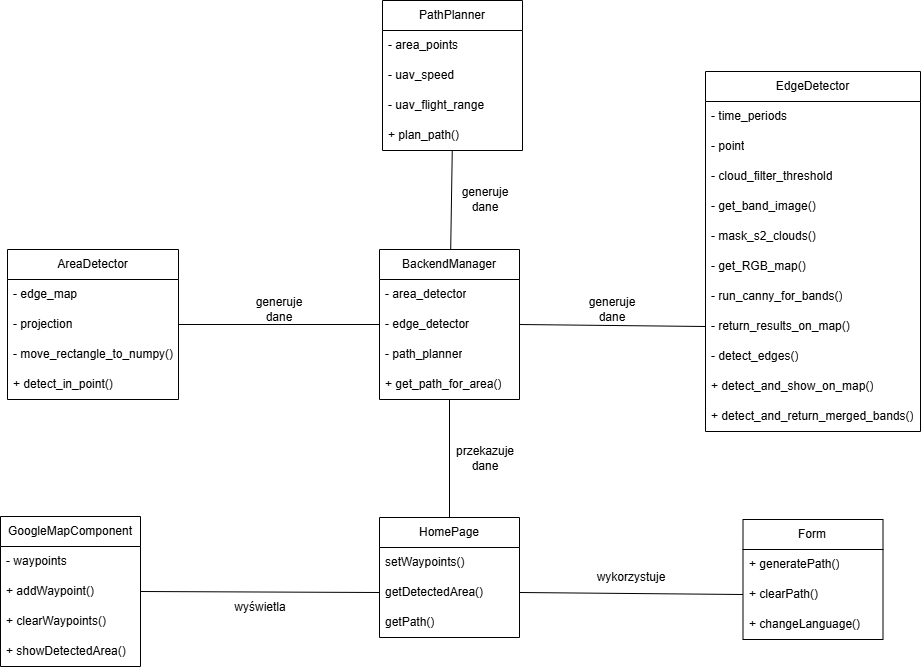
\includegraphics[width=15cm]{images/Diagram_klas.png}
    \caption{Diagram klas}
\end{figure}

Klasa BackendManager jest odpowiedzialna za przepływ sterowania podczas obsługi żądań kierowanych do backendu. Wyniki otrzymane podczas wykrywania obszarów na zdjęciach satelitarnych oraz planowania trasy do wyświetlenia będą zwracane przez tę klasę do interfejsu w celu prezentacji użytkownikowi. Ponadto, dane podane przez użytkownika będą tutaj przetwarzane i przekazywane do odpowiednich części systemu.

Klasa EdgeDetector jest odpowiedzialna za wykrywanie krawędzi na zadanym przez użytkownika obszarze. Będzie przyjmowała punkty podane przez użytkownika i następnie pobierała odpowiednie mapy i wykonywała na nich odpowiednie operacje. Otrzymane wyniki będą zwracane do klasy BackendManager.

Klasa AreaDetector wykrywa obszary na podstawie danych o wykrytych krawędziach na mapie oraz podanych przez użytkownika punktów. Wykryte obszary są przekazywane do BackendManagera w celu prezentacji ich użytkownikowi.

Klasa PathPlanner wytycza trasę przelotu drona na podstawie wykrytego obszaru przekazanego z BackendManagera. Jej wynikiem będą punkty wykrytej trasy, które będą wykorzystywane do prezentowania wyników użytkownikowi na mapie.

Komponent HomePage będzie umożliwiał użytkownikowi kierowanie żądań do backendu i zarządzanie prezentacją otrzymanych wyników podczas wykrywania obszaru i planowania trasy.

Komponent Form będzie odpowiedzialny za pobieranie od użytkownika potrzebnych do zaplanowania trasy danych.

GoogleMapComponent będzie zajmować się pobieraniem od użytkownika punktów wykorzystywanych podczas planowania trasy i wykrywania obszaru, a także prezentacją wyników poszczególnych operacji na mapie.

\subsection{Projekt interfejsu użytkownika}

Po wykonaniu specyfikacji oraz analizy wymagań względem aplikacji został wykonany projekt interfejsu użytkownika z wykorzystaniem narzędzia Figma. Całość została zaprojektowana tak, by obsługa aplikacji była uproszczona i intuicyjna, oraz by prezentowane wyniki były zrozumiałe dla użytkownika.

\begin{figure}[H]
    \centering
    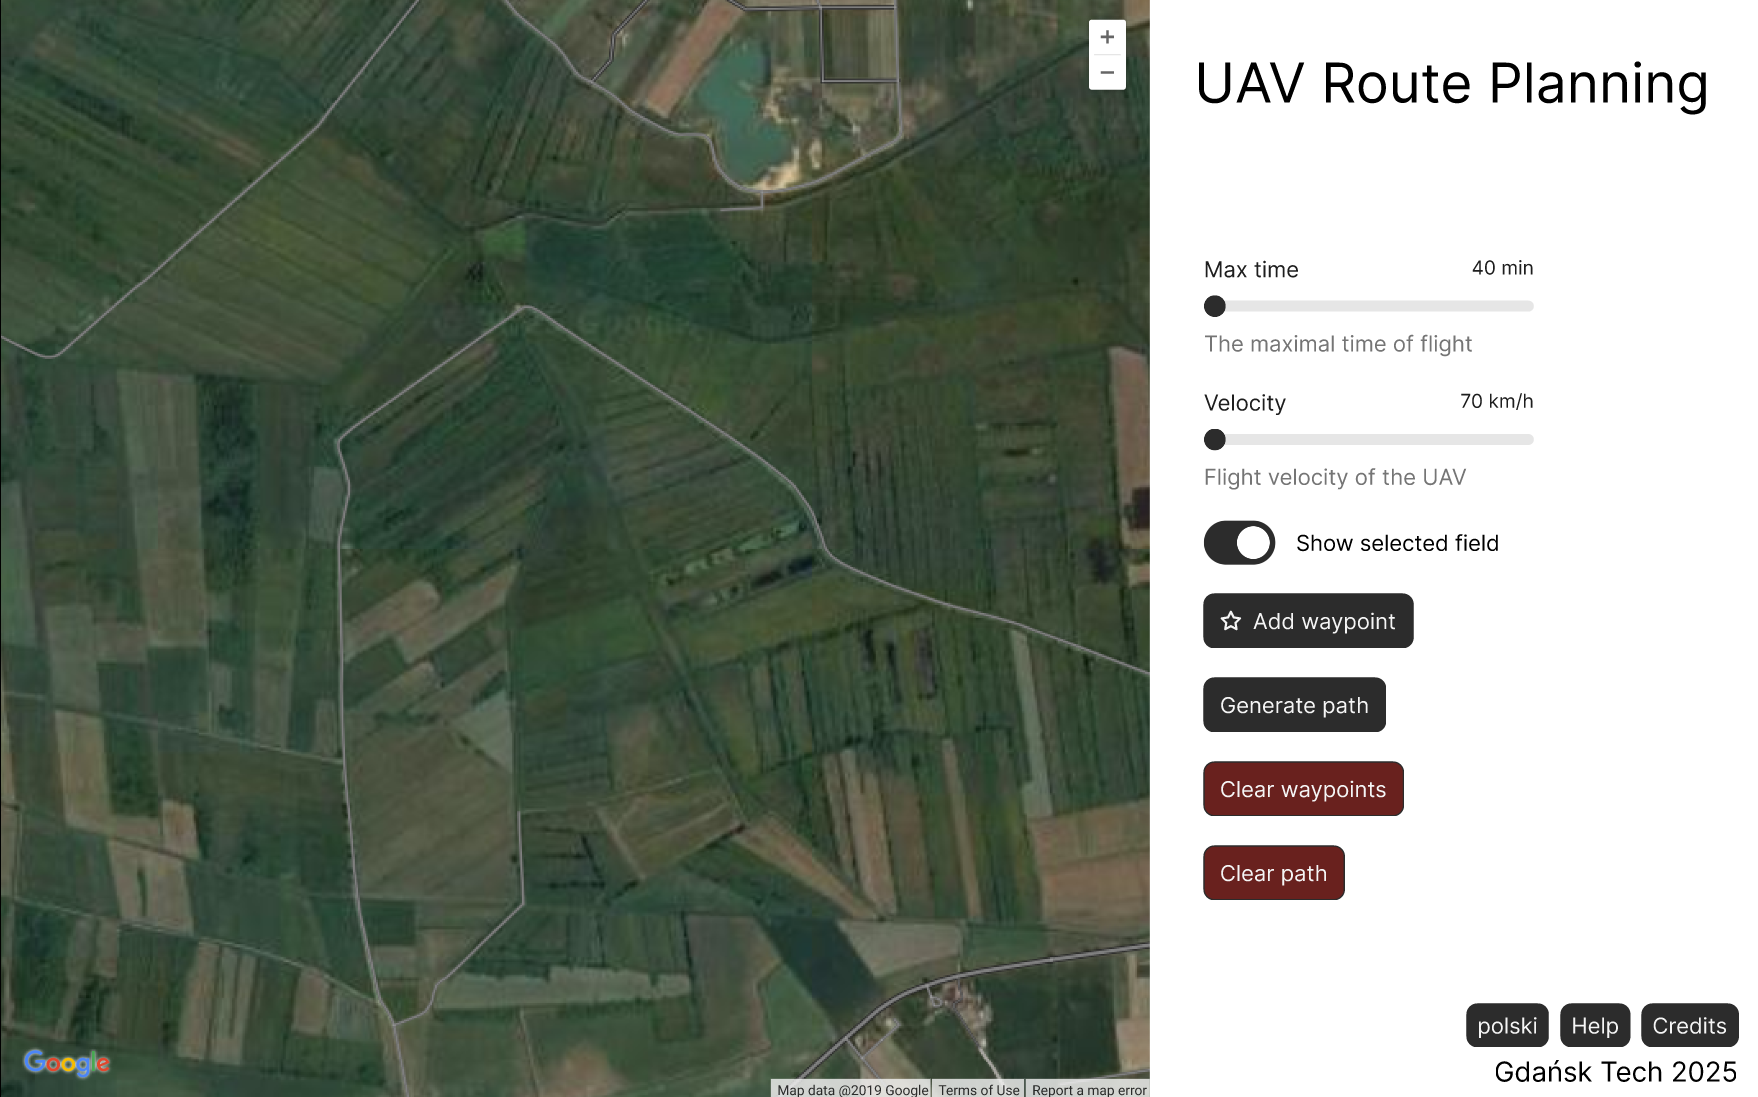
\includegraphics[width=15cm]{images/Projekt_interfejsu.png}
    \caption{Projekt interfejsu}
\end{figure}

Interfejs będzie dawał możliwość wprowadzania wymaganych do planowania trasy danych. Ponadto, po wybraniu odpowiedniej opcji będzie możliwe dodawanie punktów na mapę. Gdy użytkownik zaznaczy wszystkie punkty będzie mógł wybrać opcję planowania trasy. Jeżeli uzyskane wyniki nie będą zadowalające, możliwy będzie wybór opcji wyczyszczenia zaplanowanej trasy oraz zaznaczonych punktów na mapie. Interfejs będzie udostępniał opcję zmiany języka oraz funkcję pomocy, gdzie zostanie wyświetlony opis ułatwiający zrozumienie działania aplikacji oraz możliwe do wykonania działania.

\subsection{Wybór środowiska i implementacji}

Część aplikacji odpowiedzialna za wykrywanie krawędzi i obszarów została zaimplementowana z wykorzystaniem środowiska Colab i języka Python. Colab został wybrany z powodu łatwości w testowaniu i wizualizacji efektów osiągniętych przez zaimplementowane funkcje. Umożliwiło one łatwe porównywanie różnych parametrów rozmycia, kombinacji kanałów barw oraz różnych wartości progowania w czasie implementacji wykrywania krawędzi na obrazach.

API potrzebne do wykonywania zapytań przez interfejs użytkownika zostało zaimplementowane z wykorzystaniem środowiska PyCharm, które zostało wybrane przez zespół z powodu jego znajomości i prostoty wykorzystania. Szczególnie istotną funkcją była łatwość debugowania kodu, co w przypadku poprzedniego środowiska jest utrudnione.
Interfejs użytkownika został zaimplementowany z wykorzystaniem środowiska Visual Studio Code, które było znane członkom zespołu i jest proste w konfiguracji.

Kod projektu jest przechowywany w repozytorium GitHub, a zmiany są zapisywane w systemie kontroli wersji na bieżąco. Pozwoliło to na współpracę i dzielenie się zadaniami do wykonania oraz przeglądanie kodu i zmian na bieżąco przez każdego z członków zespołu. Dzięki komunikatom przy kolejnych wersjach zostało ułatwione utrzymanie kodu i wyłapywanie ewentualnych błędów, które pojawiły się w trakcie implementacji.

Do komunikacji w zespole był wykorzystywany Discord, na którym w razie potrzeby odbywały się spotkania zespołu w celu ustalenia planu pracy. Ponadto, w procesie wytwarzania aplikacji była wykorzystywana platforma Jira do śledzenia postępu projektu oraz tworzenia i rozdzielania zadań do wykonania, co ułatwiło dostęp do nich dla każdego z członków zespołu i uporządkowało pracę.

\subsection{Rozszerzalność aplikacji}

Aplikacja jest tworzona jako gotowy produkt umożliwiający planowanie trasy drona na wprowadzonym obszarze. Z tego powodu, prawdopodobnie nie będzie wymagała rozszerzeń w przyszłości. Mimo wszystko została ona zaprojektowana tak, że z łatwością będzie możliwe wykonanie poprawy jej funkcjonalności lub dodanie nowych.
\chapter{Implementacja, testowanie, weryfikacja i walidacja}
\label{chap:project implementation}

\section{Implementacja systemu}

\section{Testowanie}

\section{Weryfikacja założeń aplikacji}

\section{Walidacja w środowisku docelowym}
\chapter{Podsumowanie i wnioski}
\label{chap:summary}

% Bibliografia, ignorujemy overfull box, bo są długie URL
\hfuzz=50pt
\printbibliography[title=\bibliographyname]
\addcontentsline{toc}{chapter}{\bibliographyname}
\hfuzz=0pt

% Wykaz rysunków
\listoffigures
\addcontentsline{toc}{chapter}{\listfigurename}

% Wykaz tabel
\listoftables
\addcontentsline{toc}{chapter}{\listtablename}

\end{document}
